%!TEX root = Bericht.tex
\graphicspath{{graphics/}}

\chapter{Trajectory Planning}
\label{cha:trajectory}
For the two most advanced modes, i. e. the Half-Automatic and the Full-Automatic Mode, trajectories had to be generated. In this chapter the best trajectories for \textsc{Skye} are elaborated and tested with suitable trajectory controllers. Performance results based on a \textsc{Matlab} simulation are shown.

%\subsection{Our Approach}
%From the GUI it was given that the goal trajectory would be a multipoint-interpolating %trajectory. The user is able to define waypoints on a map which afterwards should be %connected with a reasonable and realizable trajectory. Beside interpolating trajectories %there exist also approximating trajectories but they were not taken into consideration, since %usually the user wants skye fly directly through a waypoint.

\section{Experimental Design}
\label{sec:experimental design}
The main application fields of the system \textsc{Skye} are image capturing and agile performance demonstrations. The waypoints used to test the trajectory algorithms had therefore to be alike these situations. All the results below belong to the three sample waypoints shown in figure \ref{fig:sampleNodes}. They represent standard situations for the applications mentioned before. Indeed, to verify the conclusions, some a wider set of waypoints had to be considered.
\\
The first waypoints are similar as they would be set to capture images of the the university building. 

\begin{figure}[h]
  \begin{minipage}[t]{0.32\textwidth}
    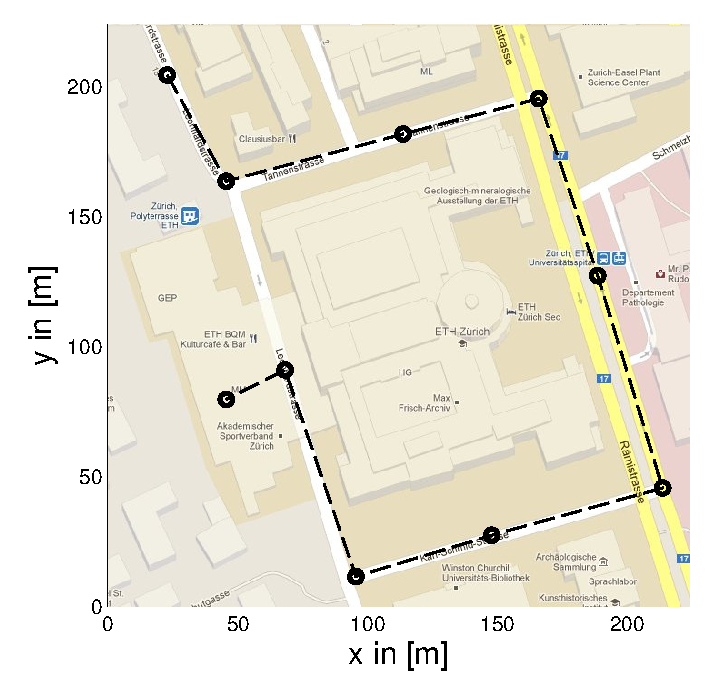
\includegraphics[width = \textwidth]{graphics/sampleNodeRoad}
  \end{minipage}
  \hfill
  \begin{minipage}[t]{0.32\textwidth}
    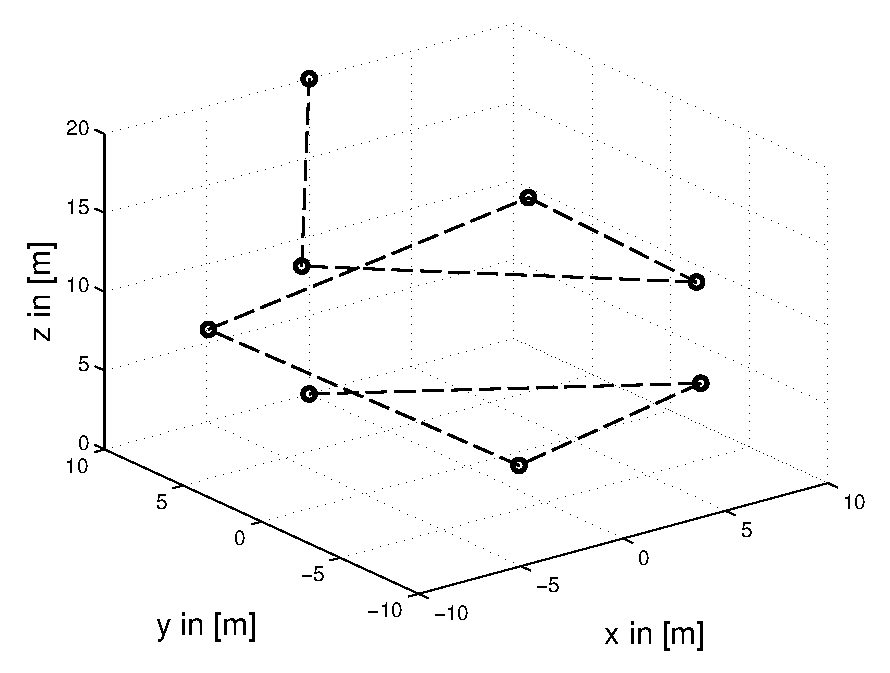
\includegraphics[width = \textwidth]{graphics/sampleNodeHelix}
  \end{minipage}
  \hfill
  \begin{minipage}[t]{0.32\textwidth}
    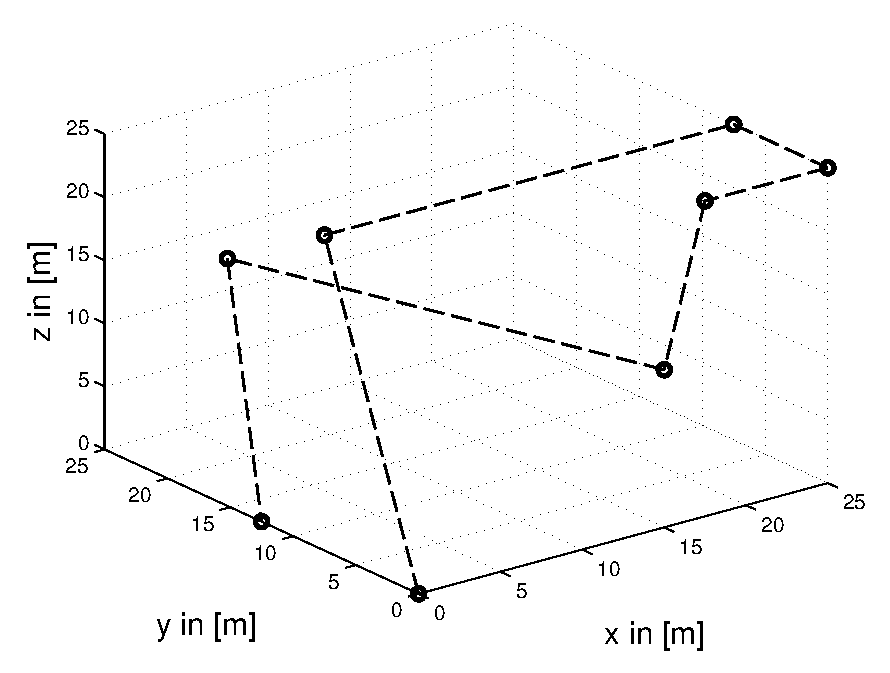
\includegraphics[width = \textwidth]{graphics/sampleNodeAgile}
  \end{minipage}
  \caption{The experimental environment based on three samples. {\bf Left:} The \textit{road} waypoints represent the need of low overshoots to not touch obstacles beside the streets. Its long straight ways enable high velocities. {\bf Center:} The \textit{helix} waypoints represents the circumnavigation of any obstacle. It yields to high curvatures of the track. {\bf Right:} The \textit{agile} waypoints include both straight sections as high curvatures.}
  \label{fig:sampleNodes}
\end{figure}


Furthermore, to score (\textbf{and optimize?}) the generated trajectories $\tilde{p}(t)$ and the resulting trace of the system $r(t)$, we set up the following criteria. Criteria (\ref{item:static_deviation}) to (\ref{item:static_acceleration}) are refered to as \textit{static criteria} as they do not depend any simulation. The remaining ones (\textit{dynamic criteria}) then mainly depend on the used controller\footnote{For detailed description of the used notation consider section \ref{sec:definition}}.
\\
Being $L_p$ the length of the path ${\bf p}(u)$ and $T_p$ the time of the trajectory $\tilde{\bf p}(t)$
\begin{equation}
L_p = \int_{u_{min}}^{u_{max}} du \qquad T_p = \int_{t_{min}}^{t_{max}} dt
\label{eq:length_of_path}
\end{equation}
the criteria are:

\begin{enumerate}[i)] 
\item Average deviation between actual path and chord (straight) connection between waypoints
\label{item:static_deviation}
\begin{equation}
J_1 = \int_{u_{min}}^{u_{max}} \|{\bf p}(u)- {\bf p}_2(u)\| du \cdot L_p^{-1} \label{eq:static_deviation}
\end{equation}

\item Average curvature of path\footnote{For a derivation of curvature see any vetor analysis book, e.g. \cite{stammbach} chapter II, page 71.}
\label{item:static_curvature}
\begin{equation}
J_2 = \int_{u_{min}}^{u_{max}} \frac{\| \frac{d {\bf p}}{du} \times \frac{d^{2} {\bf p}}{du^{2}} \|}{\|  \frac{d {\bf p}}{du} \|^3}du \cdot L_p^{-1}
\label{eq:static_curvature}
\end{equation}
% THIS ALTERNATIVE NOTATION IS INCONSEQUENCE IN USING DOT WHEN NOT HAVING PARAM T !!
% J_2 = \int_{u_{min}}^{u_{max}} \frac{\| \dot{\bf p}(u) \times \ddot{\bf p}(u) \|}{\| \dot{\bf p}(u) \|^3}du \cdot L_p^{-1}

\item Average acceleration of the trajectory
\label{item:static_acceleration}
\begin{equation}
J_3 = \int_{t_{min}}^{t_{max}} \|{\bf \ddot{\tilde{p}}}(t)\| dt \cdot T_p^{-1} \label{eq:static_acceleration}
\end{equation}

\item Deviation between trajectory and trace of the system\footnote{The deviation vector between trace and its closest point on the trajectory is always normal to the latter. Compare with figure \ref{fig:scene_crossTrack}.}
\label{item:dynamic_deviation}
\begin{equation}
J_4 = \int_{t_{min}}^{t_{max}} \| {\bf \tilde{p}}(t_{cl}) - {\bf r}(t) \| dt \cdot T_p^{-1} 
\label{eq:dynamic_deviation}
\end{equation}

\item Average acceleration of the system
\label{item:dynamic_acceleration}
\begin{equation}
J_5 = \int_{t_{min}}^{t_{max}} \|{\bf \ddot{r}}(t)\| dt \cdot T_p^{-1}
\end{equation}

\item Time synchronity\footnote{Time synchronity should be warranted for accurate \textit{trajectory} following. In our task for caputuring time independent imagery, it was only considered as a secondary aspect.}
\label{item:dynamic_synchronity}
\begin{equation}
J_6 = \| {\bf \tilde{p}}(t_{max}) - {\bf r}(t_{max}) \| \cdot L_p^{-1} \label{eq:dynamic_synchronity}
\end{equation}

\end{enumerate}


\section{Definition of Trajectories}
\label{sec:definition}
\subsection{Paths and Trajectories}
The main difference between a path $ {\bf p}(u)$ and a trajectory $ {\bf \tilde{p}}(t)$ is that only the latter includes time, i.e. considers the dynamics. A path is only defined as the way to go from point a to point b. Therefore it only has geometrical properties. In order to generate a trajectory, a time needs to be assigned to each point on the path. This is done with a function $u=u(t)$ that connects the parameter $u$ of the geometrical path with the time. The composition of the function\footnote{In  \cite{snider} named as the \textit{Motion Law}} $u=u(t)$ and the geometrical path ${\bf p}(u)$ finally forms the trajectory ${\bf \tilde{p}}(t)$. This concept is shown in figure \ref{fig:path_trajectory}.
\begin{figure}[H]
\centering
\def\svgwidth{0.9\textwidth}
\input{graphics/PathTrajectory.pdf_tex}
\caption{Composition of a path ${\bf p}(u)$ and the motion law $u(t)$ forming the trajectory ${\bf \tilde{p}}(t)$}
\label{fig:path_trajectory}
\end{figure}

In order to get the velocity and acceleration of the trajectory, the chain rule has to be applied to ${\bf \tilde{p}}(t)=({\bf p}\circ u)(t)$:

\begin{align}\label{vel_acc}
{\bf \dot{\tilde{p}}}(t) &= \frac{d {\bf p}}{du}\dot{u}(t) \\
{\bf \ddot{\tilde{p}}}(t) &= \frac{d {\bf p}}{du}\ddot{u}(t)+\frac{d^{2} {\bf p}}{du^{2}}\dot{u}^{2}(t)
\end{align}

%{\bf \ddot{\tilde{p}}}(t)





\subsection{Interpolation and Approximation}
If one wants to draw a path through a set of waypoints, there exists two ways to do this. First, the path can pass through all waypoints no matter how many bends it will have. Secondly, the path tries to best fit waypoint set, i.e. a function of a  certain order is adopted to best fit the waypoints. This can be done with different methods, e.g with least-squares. The first approach is called interpolation whereas the second approach is called approximation. Depending on the choice, different curves with different properties are formed (see figure \ref{fig:ApproxInterpol}).  


\begin{figure}[H]
  \begin{minipage}[t]{0.9\textwidth}
    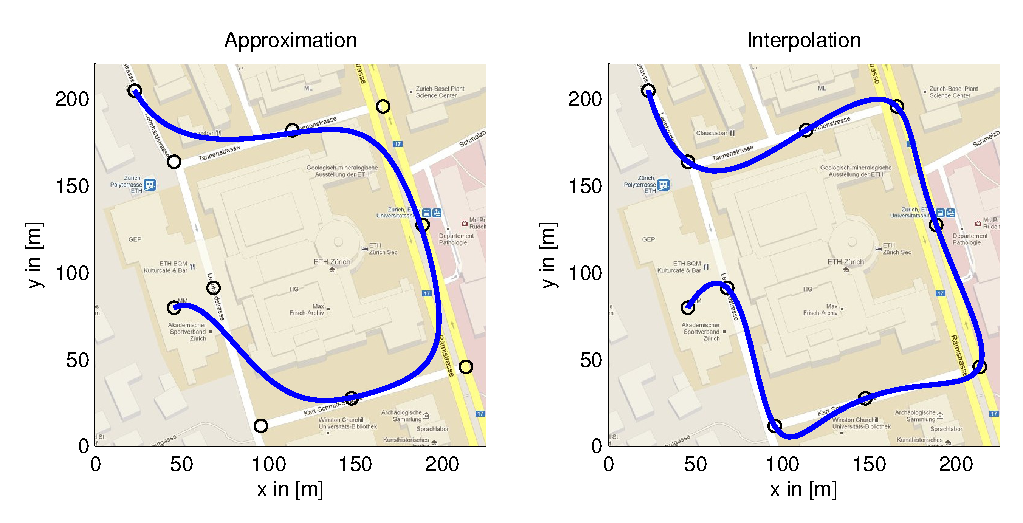
\includegraphics[width = \textwidth]{graphics/ApproxInterpol.eps}
  \end{minipage}
  \caption{Interpolation and approximation of waypoints}
  \label{fig:ApproxInterpol}
\end{figure}

For the the trajectory planning for \textsc{Skye}, it was necessary to interpolate the waypoints. This was due to the GUI used (see \ref{sec:realization}). There only a small amount of waypoints is set ant the pilot expects the UAV to pass through all of them and not to take a shortcut. The approximation of the waypoints could result in a collision with buildings as shown in \ref{fig:ApproxInterpol}.


There mainly exist two solution to interpolate a given set of $n+1$ waypoints. A polynomial (of order $\ge n+1$) from $\varPi_{n}$ or else a set of polynomials of lower order, defined over a certain interval, can be used. This set of polynomials finally forms a spline. As impressively shown in \cite{dahmen}, splines are the better option for more than a few waypoints. 



\section{Splines}
\label{sec:splines}
\subsection{Parameterization}
\label{subsec:parameterization}
Before actually a path can be drawn through a set of waypoints respectively a spline can be calculated, a value of the parameter $u$ needs to be assigned to all $n+1$ waypoints. I.e. a so called knot vector ${\bf u}$ composed of a nondecreasing sequence of $u_0 < u_1 < ...< u_n$ must be found in order to calculate a spline for each dimension.

\begin{equation}
{\bf x}(u) =  \begin{bmatrix} p_x(u) \\ p_y(u) \\p_z(u) \end{bmatrix}
   ={\bf p}(u)
\end{equation}


In this section, the most common used techniques are analyzed\footnote{A vaster evaluation of different parameterizations can be found in \cite{haron}} The choice of parameterization affects the geometrical properties of the path on the one hand and the velocity and acceleration of the trajectory on the other hand. (compare \eqref{vel_acc}). Latter is especially of big impact if a proportional relation is used to describe the motion law, i.e. $u=\lambda t$ (compare \ref{sec:motionLaw}).

\subsubsection{Uniform}
This is the simplest way to define the $u_{0-n}$. Here basically the index number of the waypoints are assigned to $u$. Therefore no meaningful interpretation can be made.
\begin{equation*}
u_n-u_{n-1}=1
\end{equation*}
\subsubsection{Chord length}
In this method the chord length between the waypoints is calculated and then summed up and assigned to $u$. With $u=\lambda t$ this method can be interpreted to aim for a more or less constant velocity over the whole trajectory.
\begin{equation*}
u_n-u_{n-1}=\left \| \begin{bmatrix}x_n\\y_n\\z_n \end{bmatrix}-\begin{bmatrix}x_{n-1}\\y_{n-1}\\z_{n-1} \end{bmatrix}\right \|
\end{equation*}
\subsubsection{Arc length}
The arc length method is improved version of the chord length distribution in order to reach a constant velocity. Here instead of taking the chord length between two waypoints, the arc length is estimated and summed up. The algorithm\footnote{The algorithm was taken from \cite{engeln} and implemented in \textsc{Matlab}.} for that can be found in \ref{subsec:arcLengthDistribution}.

\begin{figure}[h]
\centering
\def\svgwidth{0.7\textwidth}
\input{graphics/arcLength.pdf_tex}
\caption{The arc length is estimated using the segments of two circles.}
\label{fig:arcLength}
\end{figure}

\begin{equation*}
u_n-u_{n-1}=\frac{B_a+B_b}{2}
\end{equation*}

\subsubsection{Centripetal}
This method was first proposed in \cite{lee}. Here the root of the chord length is used. The motivation for this method is that the larger the angular change from $\textnormal{waypoint}_{n-1}$ to $\textnormal{waypoint}_n$, the more centripetal force is accepted. A justification for this statement can be found in \cite{doessegger} and \cite{lee}.
\begin{equation*}
u_n-u_{n-1}=\sqrt{\left \| \begin{bmatrix}x_n\\y_n\\z_n \end{bmatrix}-\begin{bmatrix}x_{n-1}\\y_{n-1}\\z_{n-1} \end{bmatrix}\right \|}
\end{equation*}

\subsubsection{Discussion}

geometrical properties, dynamical properties, Kreb'sche Bewertungsalgrithmen:) \textbf{pictures of all of them, justify choice, say that if more waypoints, different decision}

All those four methods were tested on our three sample waypoints defined in \ref{sec:experimental design}. Since the helix waypoints all have the same distance between each other, all four methods result in the same path respectively trajectory. As the chord and arc length distribution try to maintain a constant velocity, it is obvious that high curvature has to be omitted. This however leads to overshoots as seen in \ref{fig:parameterizations4_road_agile}. Choosing cubic splines reduces this effect whereas quintic splines amplifies it. (compare \ref{fig:parameterization_cqq})

\begin{figure}[H]
  \begin{minipage}[t]{0.9\textwidth}
    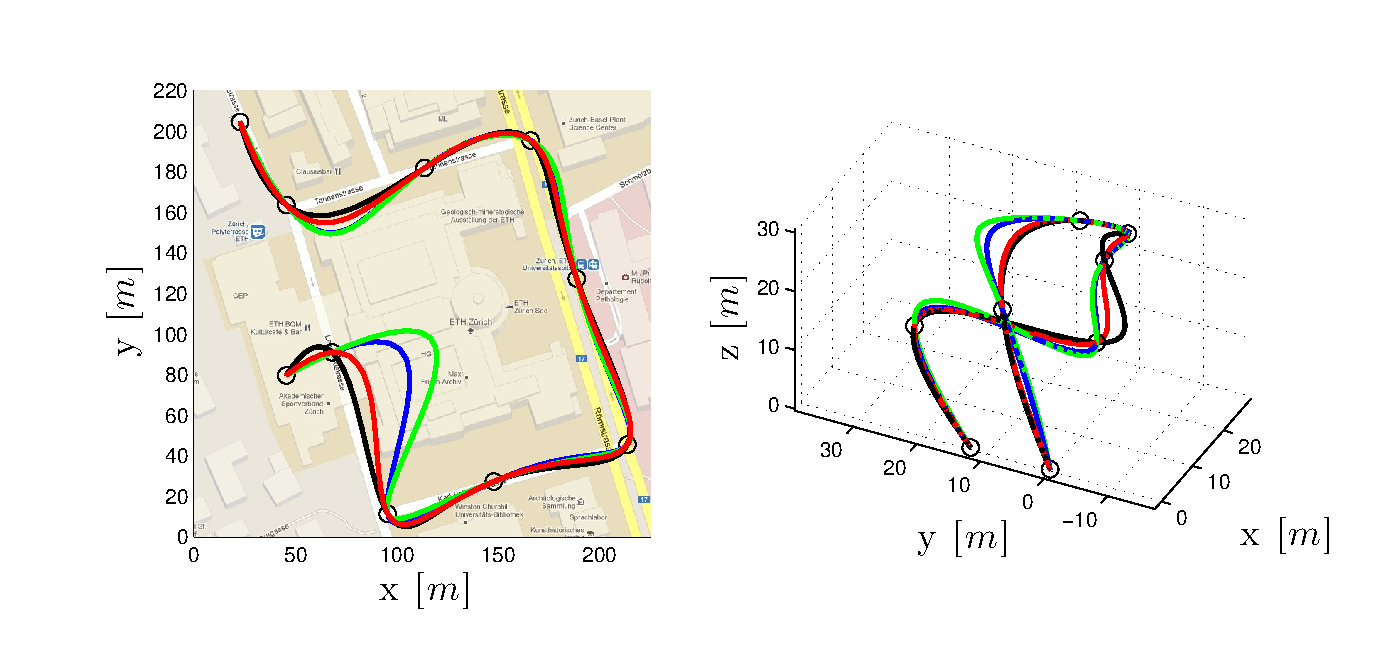
\includegraphics[width = \textwidth]{graphics/Parameterizations4_road_agile.eps}
  \end{minipage}
  \caption{The different parameterizations shown with quartic splines; Uniform: black, Chord length: blue, Arc length: green, Centripetal: red}
  \label{fig:parameterizations4_road_agile}
\end{figure}

Since those overshoots are intolerable a uniform or centripetal distribution has to be chosen. While in our sample waypoints the two seem to be quite similar the uniform distribution sometimes leads to  loops or cusps as shown in \cite{lee} and \cite{haron}. This occurs if the chord distance between the waypoints suddenly changes a lot, since the uniform distribution is completely independent of the waypoint set. Therefore the centripetal distribution was chosen to fit best our needs.
\\
Beside the geometrical appearance due to the different distributions the dynamic properties are also of big interest if a constant time scaling is used, as described in \ref{subsec:motionLaw}. Here, as the centripetal distribution is already chosen due to its geometrical properties, this is only shown for reasons of completeness. However, if the waypoints were set in a closer succession the geometrical properties would not be that important anymore and the decision should be rethought.

\begin{figure}[H]
  \begin{minipage}[t]{0.96\textwidth}
    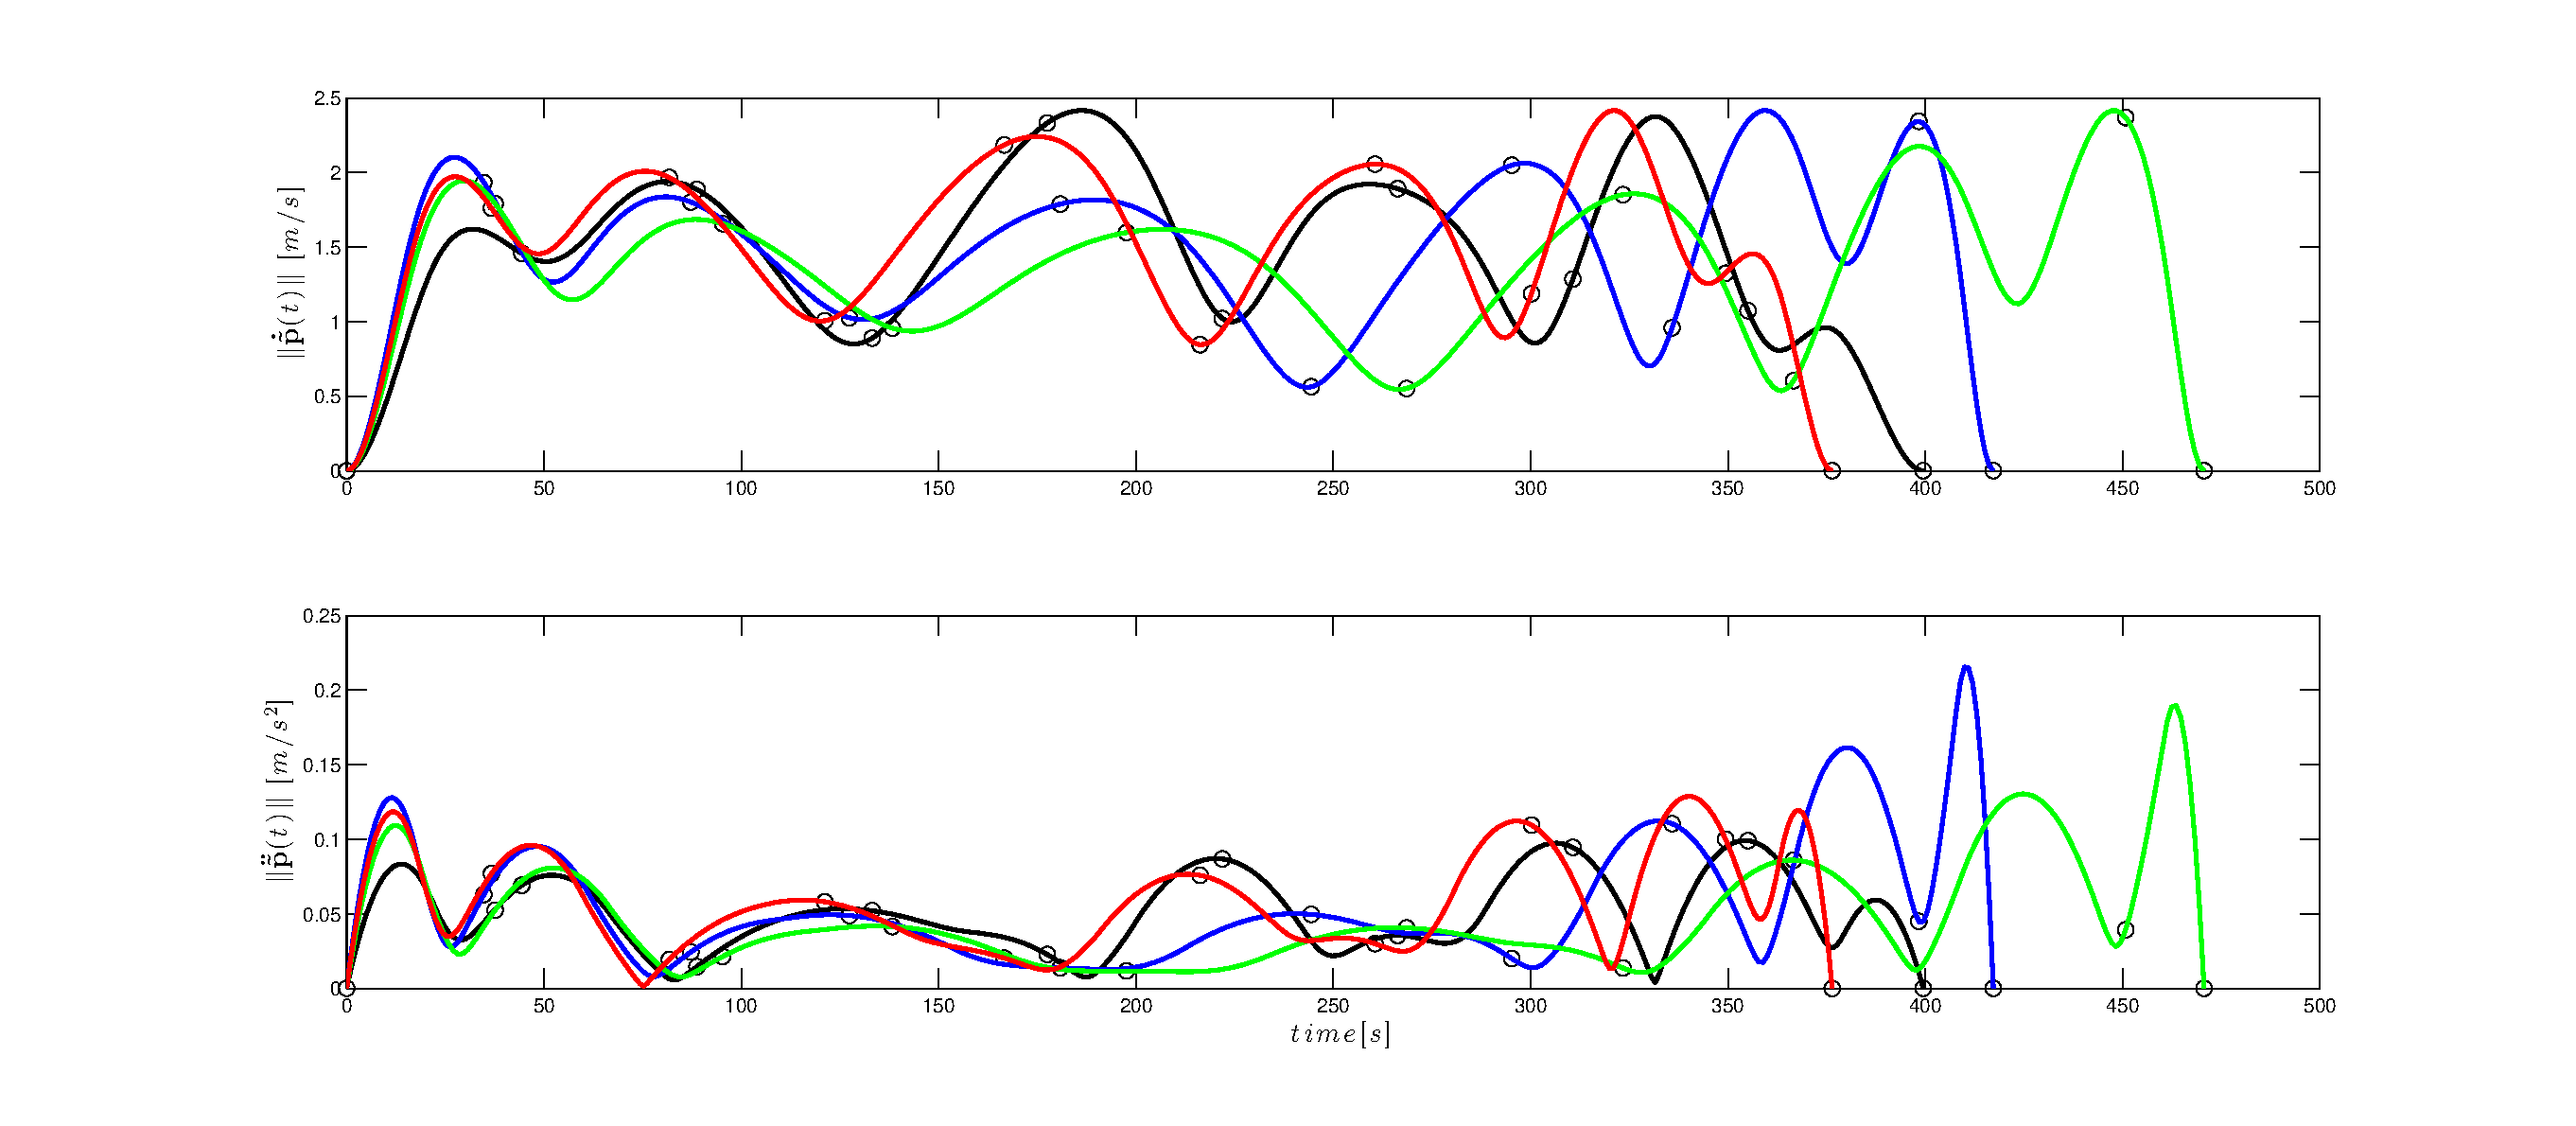
\includegraphics[width = \textwidth]{graphics/Parameterization4_road_vel_acc.eps}
  \end{minipage}
  \caption{Velocity and acceleration of the quartic road trajectory with a motion law which, in this case, limits the maximum velocity. Compare \ref{sec:motionLaw} Uniform:black, Chord length: blue, Arc length: green, Centripetal: red}
  \label{fig:para road vel acc}
\end{figure}

In figure \ref{fig:para road vel acc} the effect of the different distributions on the velocity and acceleration resulting from a constant time scaling can clearly be seen. The chord length as well as the arc length distribution keep the velocity more or less constant but start oscillating at the end of the track.

{ \bf Bring here criteria, nevertheless centripetal has to be taken anyways}


\subsection{Spline Degree}
{\bf first: explain, show continuity\\
second: Decision with Propulsion Dynamics and oscillation}
\subsubsection{Continuity}
As soon as we talk of splines the question about the spline order arises, i.e. of what degree are the polynomials which make up the spline curve. If polynomials of degree one are used then already the first derivative of the curve will not be continuous anymore. We say that this curve has a geometrical continuity of $G^0$. In the case of a trajectory the geometrical continuity of the path will directly have an influence on the continuity of the motion as can be seen from the equations \eqref{vel_acc} or in figure \ref{fig:continuity}. E. g. with a motion law of $u=\lambda t$, cubic splines are discontinuous in the jerk whereas quartic is still continuous and quintic splines would be continuous up to the snap, i.e. ${\bf \tilde{p}}(t)$ would have a parametric continuity of $C^4$ . 

\begin{figure}[H]
  \begin{minipage}[t]{0.96\textwidth}
    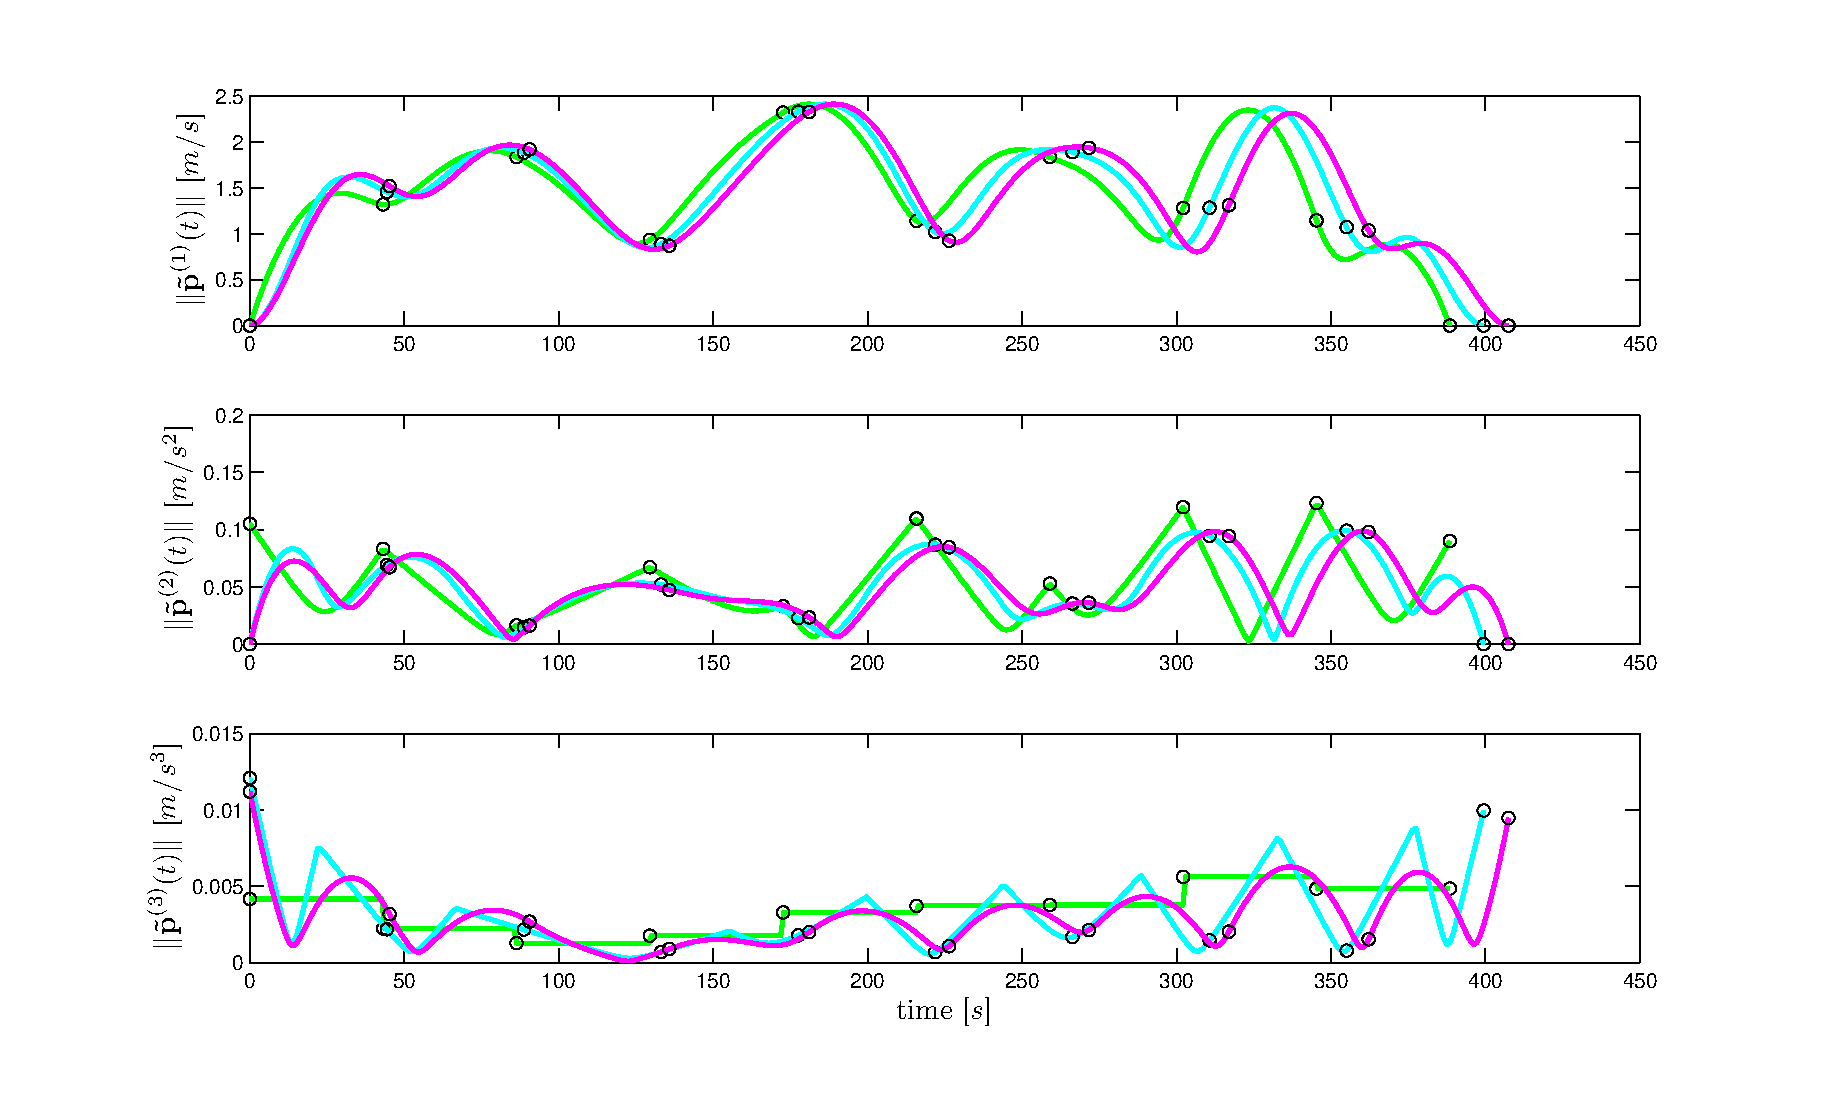
\includegraphics[width = \textwidth]{graphics/continuity.eps}
  \end{minipage}
  \caption{The different degrees of continuity for cubic (green), quartic(blue) and quintic(magenta) splines}
  \label{fig:continuity}
\end{figure}



 For \textsc{Skye} it was intuitively clear that at least cubic splines had to be used, i.e. a parametric continuity of $C^2$ was needed. This is due to its propulsion system, which is briefly described in \ref{sec:system overview} and in detail in \cite{schaffnervu}. The orientation of the thrusters cannot be turned immediately. Therefore the trajectory should not ask for a step input for the orientation of thruster which is respected by using cubic splines or splines of higher degree. However in order to find out whether even the dynamics of the thrusters or further dynamics of the positioning motor had to be considered, the whole propulsion system was fed with force calculated from the acceleration $F_x=m_{tot}a_x$. As can be seen from figure \ref{fig:forces} the propulsion system is able to handle all resulting inputs of the cubic, quartic and quintic splines.
 
\begin{figure}[H]
  \begin{minipage}[t]{0.96\textwidth}
    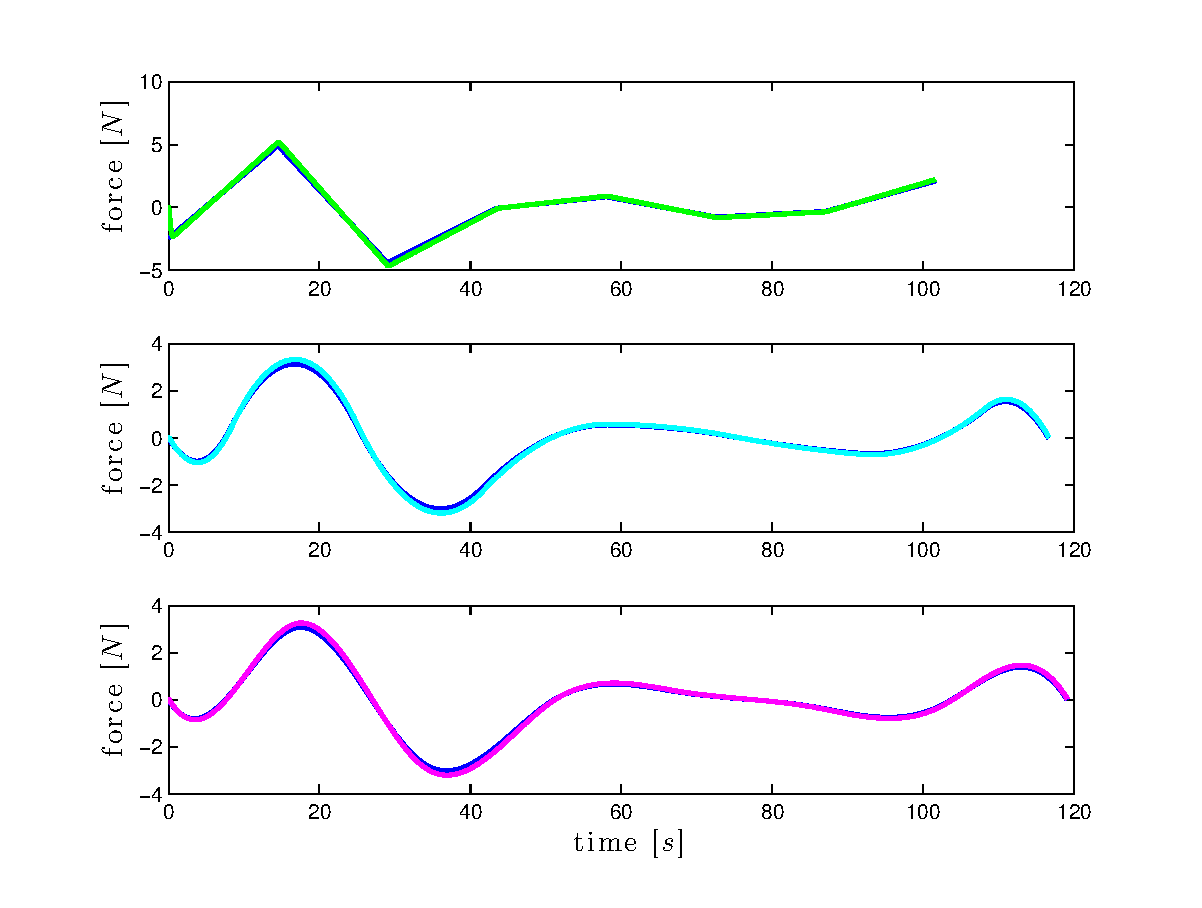
\includegraphics[width = \textwidth]{graphics/forces.eps}
  \end{minipage}
  \caption{The comparison of the forces output of the propulsion dynamics and the forces input resulting from the different degrees of splines; input:blue, output:cubic-green, quartic-blue, quintic-magenta}
\label{fig:forces}
\end{figure} 

The small deviations between the input and the output forces are a result of interpolation, done in the propulsion system \cite{schaffnervu}, and are not a result of an inadequate input. However, BLABLA.....see deviations, but much faster dynamics therefore neglectable.

{\bf here static criteria, connected with boundary conditions?}



\subsection{Boundary Conditions}
\label{subsec:boundary conditions}
{\bf v0, acc0, vn, accn null, alternative, erstes stueck der kurve durch ein polynom ersetzen.}

If $p_x(u)$ is a spline of degree $p$ and consists of $n_{knots+1}$ knots \footnote{knots are the places where the pylnominal pieces are connected}, it has $p+n_{knots}$ degrees of freedom. The polynomial of the first interval $a$ has $p+1$ degrees of freedom whereas the polynomial for the second interval $b$ is given by
\begin{equation*}
a^{j}(u_1)=b^{j}(u_1),~j=0,...,p-1
\end{equation*}
Therefore $b$ will only provide one additional degree of freedom. This is also true for all the following intervals. Therefore the spline $p_x(u)$ has finally $p+n_{knots}$ degrees of freedom\footnote{For a more mathematical proof refer to \cite{dahmen}}. Using piecewise polynomials the number of the waypoints $n+1$ is also the number of knots $n_{knots}+1$. Given the parameter $u$ for all the $n+1$ waypoints yields $p+n_{knots}-(n_{knots}+) = p-1$ constraints that still have to be imposed. As a constant time scaling is used \ref{subsec:motionLaw} it is necessary to define:

\begin{equation*}
\frac{dp_x(u)}{du} \Bigm|_{u=u_0} = \frac{dp_x(u)}{du} \Bigm|_{u=u_n}=0
\end{equation*}

in order to have the velocity at the start and at the end of the trajectory to equal zero

\begin{equation*}
\dot{\tilde{p}}_x(t_{start}) = \dot{\tilde{p}}_x(t_{end})=0
\end{equation*}

For quintic splines two additional constraints can be set

\begin{equation*}
\frac{d^2p_x(u)}{du^2} \Bigm|_{u=u_0} = \frac{d^2p_x(u)}{du^2} \Bigm|_{u=u_n}=0
\end{equation*}

such that also the acceleration at the start and at the end of the trajectory is zero(compare \eqref{vel_acc}). For quartic splines also two additional constraints can be set if B-splines are used and knots are shifted as described in \ref{subsec:implementation}. This is done for all the dimensions.



\subsection{Implementation}
\label{subsec:implementation}
As the implementation of the spline generation was not the goal of this Bsc. Thesis, it was decided to use \textsc{Matlab}'s Curve Fitting Toolbox. Yet it soon became evident that in order to correctly set correct boundary conditions for quartic and quintic splines and to get a thorough understanding it was best to program the algorithms and only use the toolbox to make the calculations with the generated splines.\\

While for the cubic splines the piecewise polynomial approach from \cite{engeln} was chosen, B-splines were chosen as a basis for the quartic and quintic splines and the proposed C-Code in \cite{biagiotti} was implemented in \textsc{Matlab} to get the B-splines and their derivatives.\\

If ${\bf u_B}=\left[u_0,...u_{n_{knots}}\right]$ is the knot vector for the B-splines, the $m=n_{knots}-p-1$ B-splines of degree $p$ for this knot vector are defined recursively using the Cox-de Boor recursion formula:

\begin{align}
B_j^0(u) &= \begin{cases} 1,&\text{if}~ u_j \leq u < u_{j+1}\\
					0,&\text{otherwise}
		\end{cases}\\
B_j^p(u) &= \frac{u-u_j}{u_{j+p}-u_j}B_j^{p-1}(u)+\frac{u_{j+p+1}-u}{u_{j+p+1}-u_{j+1}}B_{j+1}^{p-1}(u), ~p>0
\end{align}

A linear combination of B-splines then finally forms the path, whereas ${\bf c_j}$ is also referred to as control polygon:

\begin{equation}
{\bf p}(u) = \sum_{j=0}^m {\bf c_j}B_j^p(u), ~u_{mint} \leq u \leq u_{maw}
\end{equation}
 
First the knot Vector ${\bf u}$ calculated in \ref{subsec:parameterization} needs to be extended for the use with B-splines. For the quintic splines the following extension is used:
\begin{equation}
{\bf u_B}= \underbrace{ [u_0,\ldots,u_0}_{6},u_1, \ldots,u_{n-1},\underbrace{u_n,\ldots, u_n ]}_{6} 
\end{equation}
So the total number of knots is $n_{knots}+1 = n+11$ and therefore the number of the control polygon's points to be defined is $m+1=n_{knots}+1-5-1=n+5$ Given $n+1$ waypoints the 4 additional constraint on velocity and acceleration, stated in \ref{subsec:boundary conditions} are left

For the quartic splines the knot vector is shifted in order to get a better result as proposed in \cite{engeln}:
\begin{equation}
{\bf u_B}= \underbrace{ [u_0,\ldots,u_0}_{5},(u_0+u_1)/2, \ldots, (u_{k-1}-u_k)/2, \ldots,(u_{n-1}+u_n)/2,\underbrace{u_n,\ldots, u_n ]}_{5} 
\end{equation} 
Doing the same calculation as for the quintic splines here again results in $m+1=n+5$ as well, this is why the mentioned four boundary conditions in \ref{subsec:boundary conditions} hold true.

Once the knot Vector ${\bf u_B}$ is defined and the boundary conditions are set, the only thing left is to solve the following linear system of equation for all dimensions here shown for $x$:
\begin{equation}
{\bf A_{[m+1\times m+1] }}{\bf {c_x}_{[m+1\times 1]}}={\bf {b_x}_{[m+1 \times 1]}}
\end{equation}
where


\begin{equation*}
    {\bf c_x} = [ {c_x}_{0}, {c_x}_{1}, \ldots, {c_x}_{m-1}, {c_x}_{m}]
\end{equation*}

and

\begin{equation*}
{\bf A}=   \begin{bmatrix} % or pmatrix or bmatrix or Bmatrix or ...
      B_0^p(u_0)        & B_1^p(u_0)         & \ldots & B_m^p(u_0) \\
      B_0^{p(1)}(u_0) & B_1^{p(1)}(u_0) & \ldots & B_m^{p(1)}(u_0) \\
      B_0^{p(2)}(u_0) & B_1^{p(2)}(u_0) & \ldots & B_m^{p(2)}(u_0) \\
      B_0^p(u_1)         & B_1^p(u_1)         & \ldots & B_m^p(u_1) \\
      \vdots			&\vdots		     &            &\vdots \\
      B_0^p(u_{n-1})        & B_1^p(u_{n-1})         & \ldots & B_m^p(u_{n-1}) \\
      B_0^{p(2)}(u_n) & B_1^{p(2)}(u_n) & \ldots & B_m^{p(2)}(u_n) \\
      B_0^{p(1)}(u_n) & B_1^{p(1)}(u_n) & \ldots & B_m^{p(1)}(u_n) \\
      B_0^p(u_n)         & B_1^p(u_n)         & \ldots & B_m^p(u_n) \\
      
   \end{bmatrix},
   \quad 
   {\bf c_x} = \begin{bmatrix}
   {c_x}_0\\
   {c_x}_1\\
   \vdots \\
   {c_x}_{m-1}\\
   {c_x}_{m} 
    \end{bmatrix},
    \quad
   {\bf b_x} =  \begin{bmatrix}
   x_0\\
   {v_x}_0\\
   {a_x}_0\\
   x_1\\
   \vdots \\
   x_{n-1} \\
   {a_x}_n\\
   {v_x}_n\\
   x_n
    \end{bmatrix}
\end{equation*}
 






\section{Motion Law}
\label{sec:motionLaw}
\subsection{System Constraints}
\label{subsec:systemConstraints}
In order to plan a feasible trajectory one has to know the capabilities of the system. Here just a basic derivation for the velocities and accelerations is given, for more details refer to \cite{weichart}, \cite{schaffnervu}. \\

The maximum feasible acceleration in any direction is calculated to be:

\begin{equation}
  \left|a_{max} \right| =  \frac{\| {\bf F_{res, w}}\|}{m_{tot}} = \SI{0.96}{\meter\per\square\second}
\end{equation}

Whereas the $F_{res,w}$ is the force resulting from all four thrusters operated under full load in the worst direction and $m_{tot}$ is the sum of the masses of the helium, the virtual mass and the mass of the system itself.\\


The maximum feasible velocity in any direction is calculated to be:

\begin{equation}
\left|v_{max} \right| = \sqrt{\frac{\|{\bf F_{res,w}} \|}{\frac{1}{2}c_d \rho \pi r^2}}=\SI{2.9}{\meter\per\second}
\end{equation}

which is nothing but $ \left|F_{res,min} \right| = \left|F_{dray} \right| $.\\

For trajectories for position and orientation the maximal feasible angular acceleration is also important. It is calculated to be:

\begin{equation}
\left|\Psi_{max} \right| =  \frac{\| {\bf M_{res,w}}\|}{\left| \lambda_{max, J_{B}} \right|} = \SI{2.06}{\radian\per\square\second}
\end{equation}

which is quite conservative because it is assumed that worst axis for turning is also the principle axis of the inertia tensor with the highest inertia.\\

Since the system is almost undamped for rotations, the rotational velocities will never be the limiting factor.

\subsection{Motion Law}
\label{subsec:motionLaw}
Knowing the system constraints the motion law $u=u(t)$ can be defined. There are three constraints which have to be met:

\begin{itemize}
\item $u(t)$ must be monotonically increasing.
\item $u(t)$ must have a  continuity such that the composition ${\bf \tilde{p}}(t)=({\bf p}\circ u)(t)$ has the requested a parametric continuity.
\item $u(t)$ must be designed such that the trajectory ${\bf \tilde{p}}(t)$ meets the system constraints.
\end{itemize}

\begin{figure}[H]
  \begin{minipage}[t]{0.6\textwidth}
    \includegraphics[width = \textwidth]{graphics/constantTimeScaling.eps}
  \end{minipage}
  \caption{Visualization of the constant time scaling}
  \label{fig:constantTimeScaling}
\end{figure}


The most obvious solution is the one of a constant time scaling in which a constant $\lambda$ is used to scale time\footnote{It must be noticed that this is nothing but a reparameterization of the path.}.
\begin{equation}
u(t) = \lambda t
\end{equation}

In this case, $u(t)$ is monotonically increasing. And since $u(t)$ is continuous in the first derivative and for all higher derivative equal to zero, the continuity of ${\bf \tilde{p}}(t)$ only depends on on geometrical continuity of ${\bf p}(u)$ for the acceleration and higher derivatives of time.

\begin{align}
{\bf \dot{\tilde{p}}}(t) &= \frac{d {\bf p}}{du}\lambda \\
{\bf \ddot{\tilde{p}}}(t) &= \frac{d^{2} {\bf p}}{du^{2}}\lambda^2 \\
{\bf \dddot{\tilde{p}}}(t) &= \frac{d^{3} {\bf p}}{du^{3}}\lambda^3 \\
&\vdots
\end{align}

The last constraint on $u(t)$ is met with choosing $\lambda$ as follows:
\begin{equation}
\lambda = min \left\{ \frac{|v_{max}|}{\|{\bf p}^{(1)}(u)\|_{max}}, \quad \sqrt{\frac{|a_{max}|}{\|{\bf p}^{(2)}(u)\|_{max}}}  \right\}/S
\end{equation}

where $S$ is a security factor, e.g. for model uncertainties.\\
This approach of the constant time scaling is shown in figure \ref{fig:constantTimeScaling}, using an adopted visualization form \cite{doessegger}.

{\bf don't forget to mention the security factor}
{\bf show that if a polynomial is used for the first and last interval, different boundary conditions could be used}

\section{Controller Implementation}
\label{sec:controllerImplementation}
A trajectory controller and two commonly used path tracking controllers\footnote{\cite{snider} provides a good overview to various approaches.} are tested to follow the defined trajectories. The \textit{trajectory following} controller supplies the system's position controller \cite{meiermueri} with a feed forward reference signal. Although it delivers good results for ideal case, the tracking get worse for the non perfect model case. The \textit{pure pursuit} controller, which is based on a lookahead point as well as the \textit{cross track error} controller dynamically react on model uncertainties and yield therefore to more robust and accurate path tracking results.
SOMEWHERE PROBABLY CITE \cite{deluca}
\subsection{Trajectory following}
Assuming a perfect model and a trajectory considering all system constraints\footnote{I.e. saturations of $\dot{r}(t)$ and its derivatives, see section \ref{subsec:systemConstraints}.} the position $r\left(t\right)$ of the system can be assumed to be equal to the trajectory $\tilde{p}(t)$ at any time. Therefore, a straight forward way of a trajectory controller is to follow the trajectory $\tilde{p}(t)$ for every time $t$. This yields to accurate tracking in a safe environment \cite{doessegger}.
\\
A position PI controller with feedforward terms for velocity and acceleration as described in \cite{meiermueri} can therefore be used with the reference input

\begin{equation}
  [r_{ref}(t), \; \dot{r}_{ref}(t), \; \ddot{r}_{ref}(t)]^T = [\tilde{p}(t), \; \dot{\tilde{p}}(t), \; \ddot{\tilde{p}}(t)]^T
\end{equation}

The controller scheme is shown in figure \ref{fig:trajectoryfollowing}. 

%$\left[ \begin{array}{c} {\bf r}(t) \\ {\bf \dot{r}}(t) \end{array} \right]$
\begin{figure}[H]
    \centering
    \def\svgwidth{0.4\columnwidth}
    \input{graphics/scene_trajectoryFollowing.pdf_tex}
    \caption{Trajectory Following. The reference state is predefined by the trajectory for every time $t$.}
    \label{fig:scene_trajectoryFollowing}
\end{figure}

\begin{figure}[H]
    \centering
    \def\svgwidth{\columnwidth}
    \input{graphics/controller_trajectoryFollowing.pdf_tex}
    \caption{Trajectory following controller. The value of the parameter $t$ of the trajectory is equal to the current time.}
    \label{fig:trajectoryfollowing}
\end{figure}

%\begin{figure}[h]
%    \centering
%    \includegraphics[width = \textwidth]{trackings/figure_2D_road_SplineDegree3_trajectoryFollowing_Disturbance_0}
%  \hfill
%  \caption{BLA dynamics}
%  \label{fig:trajFoll_dynamics}
%\end{figure}

%\begin{figure}[h]
%    \centering
%    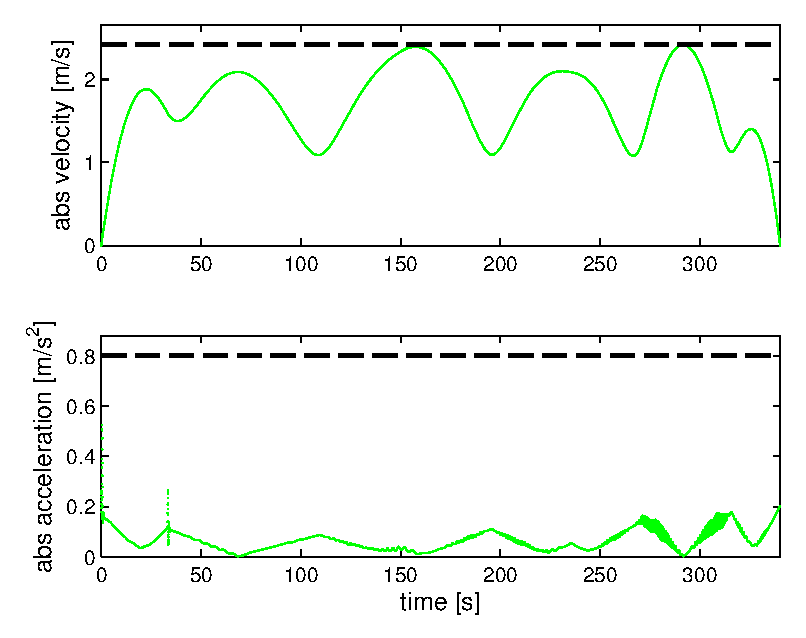
\includegraphics[width = 0.8\textwidth]{trackings/figure_1D_road_SplineDegree3_trajectoryFollowing_Disturbance_0}
%  \hfill
%  \caption{BLA dynamics}
%  \label{fig:trajFoll_dynamics}
%\end{figure}

\subsection{Pure Pursuit Controller}
Another commonly used controller to track paths is \textit{Pure Pursuit} \cite{snider}. This technique is mainly used for path tracking only with a e.g. constant given tangential velocity. The idea of using a lookahead point was adapted for trajectory control. To do that, the lookahead point is set on the trajectory $\Delta T$\footnote{$\Delta T = \SI{1}{second}$ proofed to be reasonable for all considered conditions.} in front of the current closest position ${\bf \tilde{p}}(t_{cl})$.
\begin{equation}
\tilde{p}(t_{cl}+\Delta T) = {\bf \tilde{p}}(t_{cl}) + \Delta T \cdot {\bf\dot{ \tilde{p}}}(t_{cl}) + \frac{1}{2} \Delta T^2 \cdot {\bf\ddot{ \tilde{p}}}(t_{cl}) + \mathcal{O}(\Delta T^3)
\end{equation}
Therefore, the controller considers the full dynamics of the trajectory, i.e. ${\bf \tilde{p}}(t)$ and all its derivatives\footnote{This is a simple and robust alternative to any derivative controller.}.
Figure \ref{fig:scene_purePursuit} represents the controllers functionality. The control scheme can be seen in figure \ref{fig:purePursuit}. Actually, the inner control block is a velocity controller only. The reference velocity is given by
\begin{equation}
{\bf \dot{r}}_{ref}(t) = \frac{{\bf \tilde{p}}(t_{cl}+\Delta T)-{\bf r}(t)}{\Delta T}
\end{equation}


%$ {\bf \dot{r}}_{ref}(t) $
\begin{figure}[H]
    \centering
    \def\svgwidth{0.5\columnwidth}
    \input{graphics/scene_purePursuit.pdf_tex}
    \caption{Pure pursuit. The reference velocity is given by the difference between the actual position and a lookahead defined by the trajectory $\Delta T$ ahead the closest point.}
    \label{fig:scene_purePursuit}
\end{figure}

\begin{figure}[H]
    \centering
    \def\svgwidth{\columnwidth}
    \input{graphics/controller_purePursuit.pdf_tex}
    \caption{Pure pursuit controller. The position feedback is closed by defining the lookahead point depending on the closest point of the trajectory.}
    \label{fig:purePursuit}
\end{figure}

%\begin{figure}[H]
%  \begin{minipage}[t]{0.32\textwidth}
%    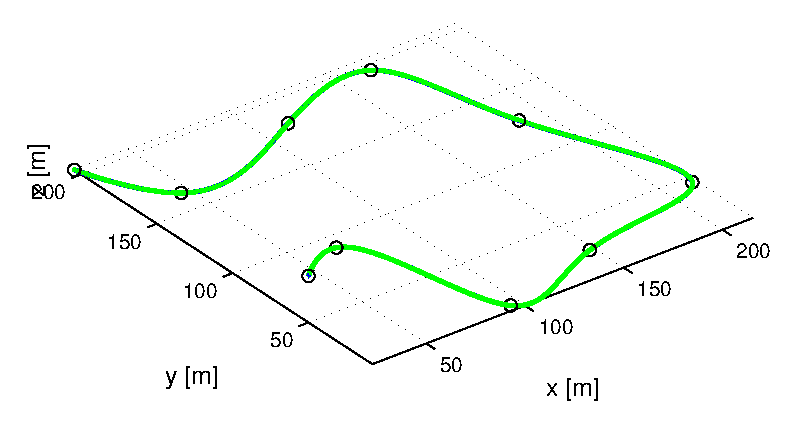
\includegraphics[width = \textwidth]{trackings/figure_3D_road_SplineDegree3_purePursuit_Disturbance_0}
%  \end{minipage}
%  \hfill
%  \begin{minipage}[t]{0.32\textwidth}
%    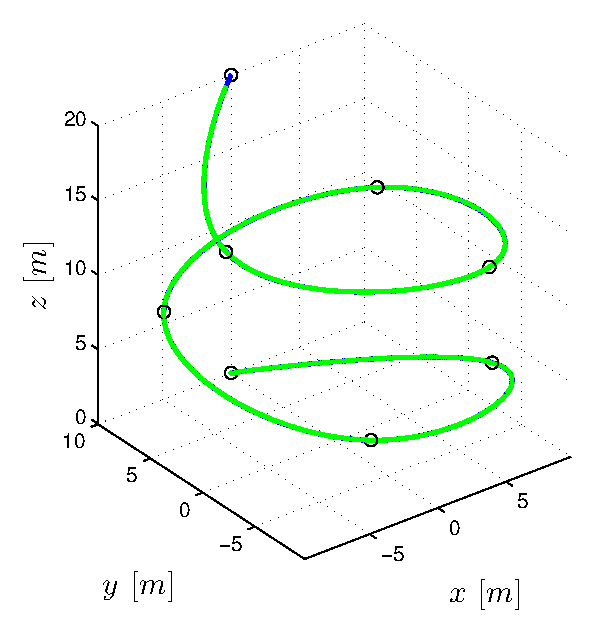
\includegraphics[width = \textwidth]{trackings/figure_3D_helix_SplineDegree3_purePursuit_Disturbance_0}
%  \end{minipage}
%  \hfill
%  \begin{minipage}[t]{0.32\textwidth}
%    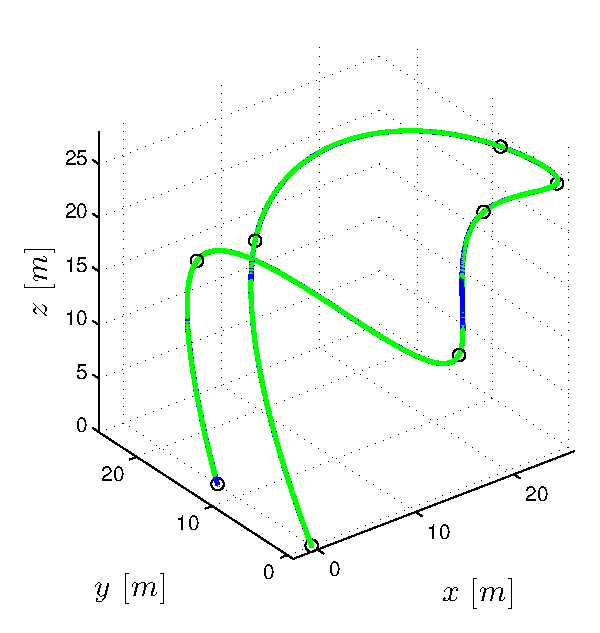
\includegraphics[width = \textwidth]{trackings/figure_3D_agile_SplineDegree3_purePursuit_Disturbance_0}
%  \end{minipage}
%  \caption{BLA pure pursuit}
%  \label{fig:purePursuit_tracking}
%\end{figure}
%
%\begin{figure}[H]
%  \begin{minipage}[t]{0.32\textwidth}
%    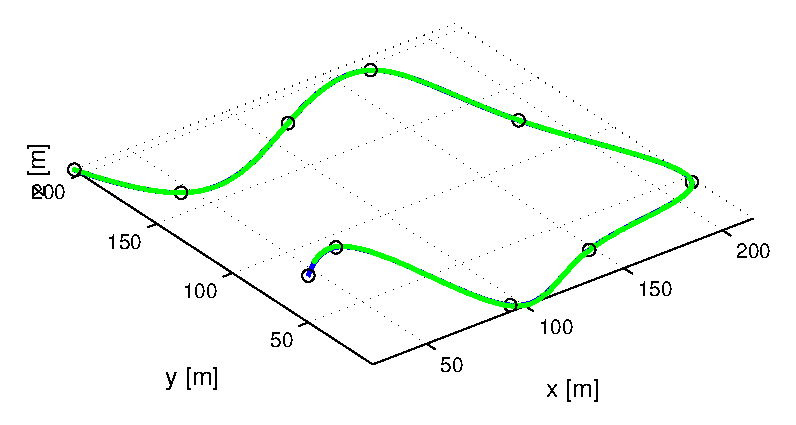
\includegraphics[width = \textwidth]{trackings/figure_3D_road_SplineDegree3_purePursuit_Disturbance_1}
%  \end{minipage}
%  \hfill
%  \begin{minipage}[t]{0.32\textwidth}
%    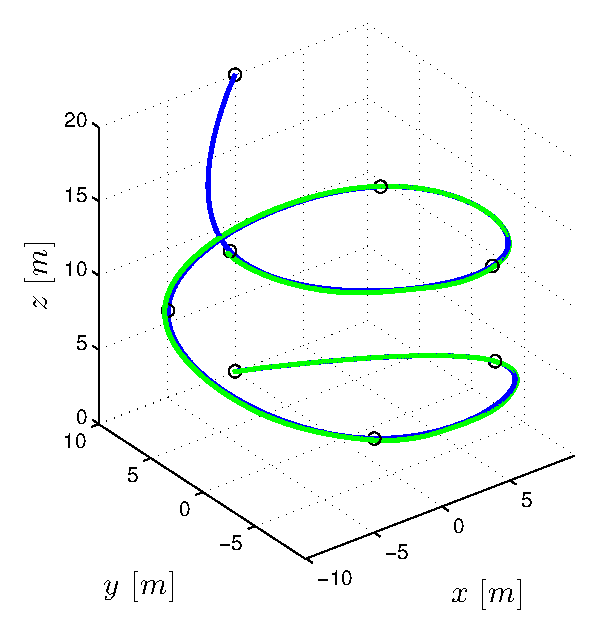
\includegraphics[width = \textwidth]{trackings/figure_3D_helix_SplineDegree3_purePursuit_Disturbance_1}
%  \end{minipage}
%  \hfill
%  \begin{minipage}[t]{0.32\textwidth}
%    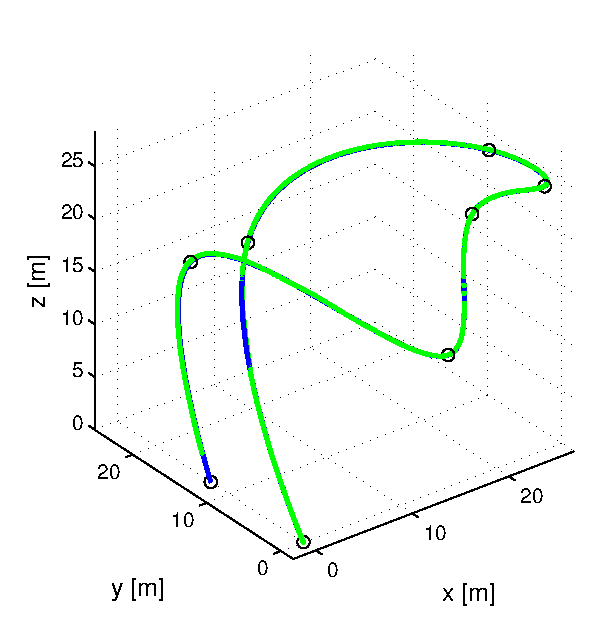
\includegraphics[width = \textwidth]{trackings/figure_3D_agile_SplineDegree3_purePursuit_Disturbance_1}
%  \end{minipage}
%  \caption{BLA pure pursuit and here with wind}
%  \label{fig:purePursuit_tracking}
%\end{figure}

\subsection{Cross Track Error Controller}
The idea of the \textit{cross track error} controller is to directly reduce the cross track distance. This practise is also used in navy \cite{williams} or for wheeled robots \cite{deluca}. The actual operation is very similar to the one in \textit{trajectory following}, but instead of taking the trajectory's current time, here the reference input time is defined by the closest point of the trajectory. Afterwards, the same position controller as mentioned above is used to track the reference state. Figure \ref{fig:scene_crossTrack} illustrates the choise of the reference input for the controller. The control scheme is shown in figure \ref{fig:crossTrack}.

%$\left[ \begin{array}{c} {\bf \tilde{p}}(t) \\ {\bf \dot{\tilde{p}}}(t) \\ {\bf \ddot{\tilde{p}}}(t) \end{array} \right]$
\begin{figure}[H]
    \centering
    \def\svgwidth{0.5\columnwidth}
    \input{graphics/scene_crossTrack.pdf_tex}
    \caption{Cross track error. The reference point is the nearest point on the trajectory.}
    \label{fig:scene_crossTrack}
\end{figure}


\begin{figure}[H]
    \centering
    \def\svgwidth{\columnwidth}
    \input{graphics/controller_crossTrack.pdf_tex}
    \caption{Cross track error controller. The value of the trajectories time stamp $t_{cl}$ of the closest point is generally not equal the current time $t$.}
    \label{fig:crossTrack}
\end{figure}


%\begin{figure}[H]
%  \begin{minipage}[t]{0.32\textwidth}
%    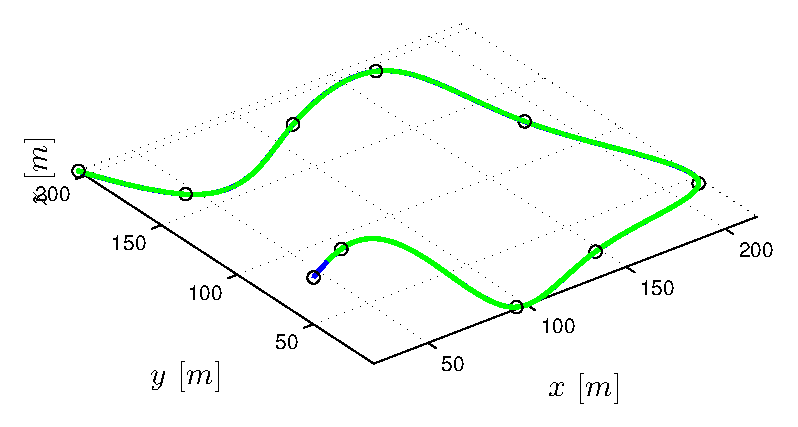
\includegraphics[width = \textwidth]{trackings/figure_3D_road_SplineDegree3_crossTrack_Disturbance_0}
%  \end{minipage}
%  \hfill
%  \begin{minipage}[t]{0.32\textwidth}
%    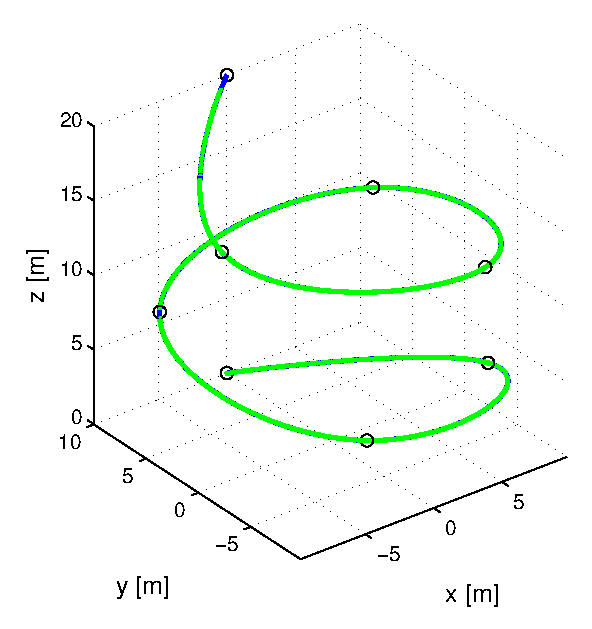
\includegraphics[width = \textwidth]{trackings/figure_3D_helix_SplineDegree3_crossTrack_Disturbance_0}
%  \end{minipage}
%  \hfill
%  \begin{minipage}[t]{0.32\textwidth}
%    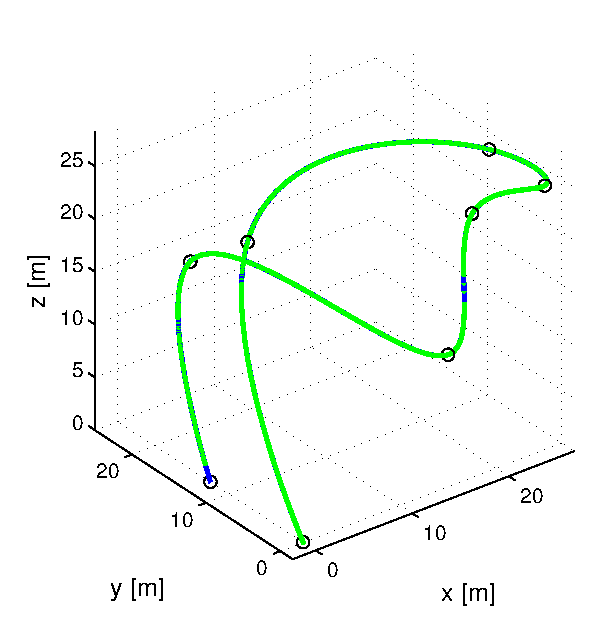
\includegraphics[width = \textwidth]{trackings/figure_3D_agile_SplineDegree3_crossTrack_Disturbance_0}
%  \end{minipage}
%  \caption{BLA cross track}
%  \label{fig:crossTrack_tracking}
%\end{figure}
%
%\begin{figure}[H]
%  \begin{minipage}[t]{0.32\textwidth}
%    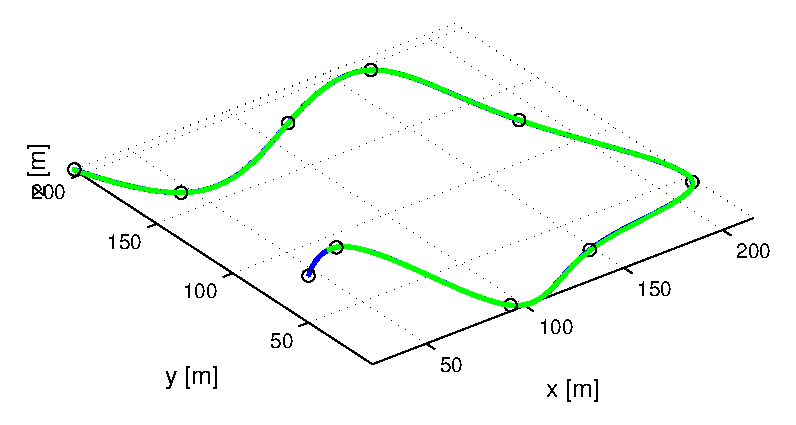
\includegraphics[width = \textwidth]{trackings/figure_3D_road_SplineDegree3_crossTrack_Disturbance_1}
%  \end{minipage}
%  \hfill
%  \begin{minipage}[t]{0.32\textwidth}
%    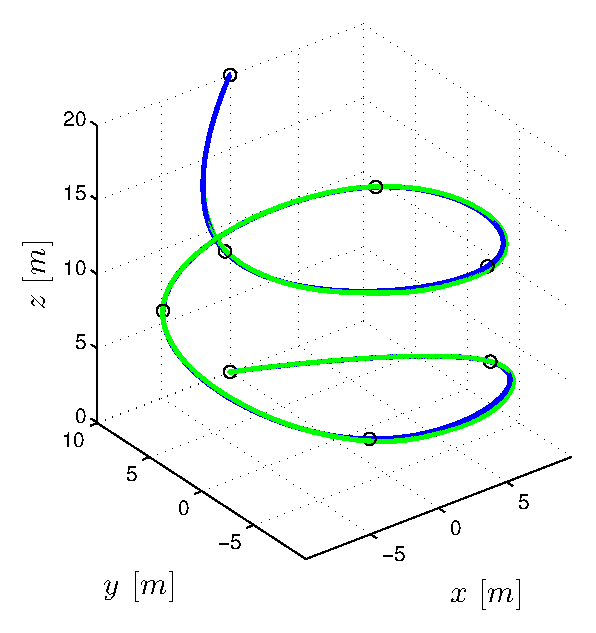
\includegraphics[width = \textwidth]{trackings/figure_3D_helix_SplineDegree3_crossTrack_Disturbance_1}
%  \end{minipage}
%  \hfill
%  \begin{minipage}[t]{0.32\textwidth}
%    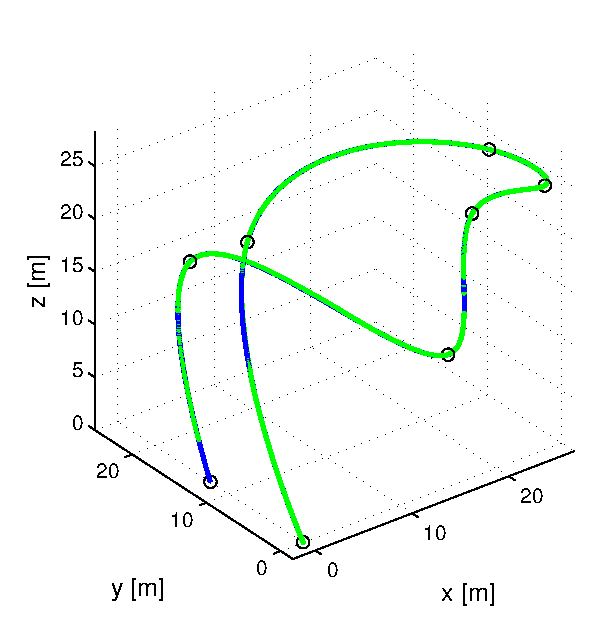
\includegraphics[width = \textwidth]{trackings/figure_3D_agile_SplineDegree3_crossTrack_Disturbance_1}
%  \end{minipage}
%  \caption{BLA cross track with wind}
%  \label{fig:crossTrackWind_tracking}
%\end{figure}

\section{Results}
\label{sec:results}

A model of system \textsc{Skye} has been elaborated in \cite{weichart} and was available as \textsc{Matlab Simulink} model to test the controller performance. The controllers described above were tested within the experimental design notified in section \ref{sec:experimental design}. If not mentioned explicitly, the shown trajectories are designed using cubic splines and centripetal parametrization. The results are presented for perfect model estimation as well as wind disturbance and model uncertainties. Furthermore the correlation between different parameters is exposed. Further results can be found in the Appendix (\ref{sec:app_trajectory_control_results}).

\subsection{Perfect Model Estimation}
\label{sub:results_perfect_model}

The three trajectory controllers were tested on the given conditions. Figure \ref{fig:results_perfect_model} shows their tracking. The performance difference between them is minimal as it can be seen from the results listed in table \ref{tab:results_perfect_model}. In comparison to the systems characteristic size (diameter \SI{2.7}{\meter}) the deviations between trajectory and trace are extremely small, i.e. less than 1\% of the characteristic size. 

\begin{table}[h]
\begin{center}
 \begin{tabular}{lll|rrr}
 \hline
 Controller &   & unit & \textit{Road} & \textit{Helix} & \textit{Agile} \\ \hline \hline
 Trajectory Following & Av. Dev. & $[\si{\meter}]$ & 0.007 & 0.017 & 0.014 \\
 Pure Pursuit         & Av. Dev. & $[\si{\meter}]$ & 0.007 & 0.009 & 0.017 \\
 Cross Track          & Av. Dev. & $[\si{\meter}]$ &  0.007 & 0.007 & 0.006 \\
    
 Trajectory Following & Av. Acc. & $[\si{\meter\per\square\second}]$ & 0.029 & 0.174 & 0.137 \\
 Pure Pursuit         & Av. Acc. & $[\si{\meter\per\square\second}]$ & 0.031 & 0.159 & 0.128 \\
 Cross Track          & Av. Acc. & $[\si{\meter\per\square\second}]$ & 0.029 & 0.159 & 0.126 \\
 
 Trajectory Following & Reached & $[\si{\percent}]$ & 100 & 100 & 100 \\
 Pure Pursuit         & Reached & $[\si{\percent}]$ &  99 &  97 &  98 \\
 Cross Track          & Reached & $[\si{\percent}]$ &  97 &  97 &  97 \\
 \hline
 \end{tabular}
 \caption{Results of the three controllers using perfect model estimation}\vspace{1ex}
 \label{tab:results_perfect_model}
\end{center}
\end{table}


\subsection{Wind Disturbance}
\label{sub:results_wind_disturbance}

The same simulations have been conducted with wind disturbance. Wind forces based on a constant wind velocity of \SI{1}{\meter\per\second} in positive x-direction have been added to the scenes. The disturbance is added 10 seconds after the simulation's start. \\
Figure \ref{fig:results_wind_disturbance} shows the tracking reached by the three controllers. The resulting performance values are listed in table \ref{tab:results_wind_disturbance}. While \textit{pure pursuit} and \textit{cross track error} control remain small deviation\footnote{They are still about factor 20 smaller than the characteristic size of \textsc{Skye}.} it has grown to aconsiderable big scale for \textit{trajectory following}. \textit{Cross track error} control slightly scores better than \textit{pure pursuit}. Again, the accelerations are similar for all controllers. While \textit{trajectoy follwing} reaches the end of the trajectory within the given time $T_p$ by definition, the path tracking based trajectory controllers will remain at \SIrange{86}{96}{\percent} of the trajectories length $L_p$ at the time $T_p$. \\
Compared to the results of perfect modelling, the deviations of the accurate controllers get worse \numrange{5}{10} times and of \textit{trajectory following} by factor \numrange{10}{200}. The accelerations are comparable to the ideal case. 

\begin{table}[h]
\begin{center}
 \begin{tabular}{lll|rrr}
 \hline
 Controller &   & unit & \textit{Road} & \textit{Helix} & \textit{Agile} \\ \hline \hline
 Trajectory Following & Av. Dev. & $[\si{\meter}]$ & 1.783 & 0.606 & 0.111 \\
 Pure Pursuit         & Av. Dev. & $[\si{\meter}]$ & 0.079 & 0.098 & 0.037 \\
 Cross Track          & Av. Dev. & $[\si{\meter}]$ & 0.034 & 0.061 & 0.023 \\

 Trajectory Following & Av. Acc. & $[\si{\meter\per\square\second}]$ & 0.031 & 0.191 & 0.138 \\
 Pure Pursuit         & Av. Acc. & $[\si{\meter\per\square\second}]$ & 0.031 & 0.136 & 0.121 \\
 Cross Track          & Av. Acc. & $[\si{\meter\per\square\second}]$ & 0.028 & 0.140 & 0.120 \\
 
 Trajectory Following & Reached & $[\si{\percent}]$ & 100 & 100 & 100 \\
 Pure Pursuit         & Reached & $[\si{\percent}]$ &  96 &  86 &  96 \\
 Cross Track          & Reached & $[\si{\percent}]$ &  94 &  89 &  95 \\
 \hline
 \end{tabular}
 \caption{Results of the three controllers with wind disturbance}\vspace{1px}
 \label{tab:results_wind_disturbance}
\end{center}
\end{table}


\subsection{Model Uncertainties}
\label{sub:results_model_uncertainties}

The simulations were repeated by designing the trajectories by system constraints with a safety factor reduced to less than one, i.e. to \num{0.8}. Therefore, the trajectory overestimates the system's actuation possibilities. \\
The tracking of all controllers is shown in figure \ref{fig:results_model_uncertainties}. The numerical results are listed in table \ref{tab:results_model_uncertainties}. The deviation of \textit{trajectory following} control is considerable larger than of the two other ones. \textit{Pure pursuit} even beats the \textit{cross track error} results. The average accelerations are slightly higher when using \textit{trajectory follwing}. Contrary to the \textit{trajectory following} that heads to the actual end of the trajectory by $T_p$, \textit{pure pursuit} and \textit{cross track error} will lead to \SIrange{86}{93}{\percent} of the circuit's length.
\\
In comparison to the ideal case, the deviations of the accurate controllers get worse \numrange{2}{10} times. \textit{Trajectory following} lead to deviations \numrange{50}{400} times larger than for perfect modelling. Average accelerations grew by factors less than \num{2}.

\begin{table}[h]
\begin{center}
 \begin{tabular}{lll|rrr}
 \hline
 Controller &   & unit & \textit{Road} & \textit{Helix} & \textit{Agile} \\ \hline \hline
 Trajectory Following & Av. Dev. & $[\si{\meter}]$ & 3.228 & 1.628 & 0.838 \\
 Pure Pursuit         & Av. Dev. & $[\si{\meter}]$ & 0.049 & 0.026 & 0.036 \\
 Cross Track          & Av. Dev & $[\si{\meter}]$ &  0.092 & 0.044 & 0.058 \\
    
 Trajectory Following & Av. Acc. & $[\si{\meter\per\square\second}]$ & 0.066 & 0.234 & 0.234 \\
 Pure Pursuit         & Av. Acc. & $[\si{\meter\per\square\second}]$ & 0.045 & 0.210 & 0.182 \\
 Cross Track          & Av. Acc. & $[\si{\meter\per\square\second}]$ & 0.047 & 0.220 & 0.192 \\
 
 Trajectory Following & Reached & $[\si{\percent}]$ & 100 & 100 & 100 \\
 Pure Pursuit         & Reached & $[\si{\percent}]$ &  86 &  90 &  86 \\
 Cross Track          & Reached & $[\si{\percent}]$ &  87 &  93 &  89 \\
 \hline
 \end{tabular}
 \caption{Results of the three controllers with underestimated trajectory constraints}\vspace{1px}
 \label{tab:results_model_uncertainties}
\end{center}
\end{table}

\subsection{Data Correlation}
Within the gathered data for the tracking with ideal conditions (section \ref{sub:results_perfect_model}) and considering all introduced parametrizations and spline degrees from section \ref{sec:splines} a data set of 108 items was analyzed for correlation\footnote{The additional cases with non perfect modelling ($3\cdot 108$ items with wind and/or model uncertainties) will not be shown. Indeed, the correlations cannot be seen there explicitly}. Some correlating results could be observed. \\
Figure \ref{fig:correlation_time_acc} shows the relation between the given time $T_p$ for the trajectory and the average acceleration $J_5$ occurring on the system. The result is trivial, as the less time is given to follow the waypoints, the higher gets the acceleration. The dependence on the used parametrization is different for the different waypoints, whereas higher spline degrees (quartic and quintic) yield to slightly smaller time $T_p$ and acceleration $J_5$ than lower degree (cubic) consequently. \\
In figure \ref{fig:correlation_invdev_acc} the correlation between average deviation $J_4$ and the average acceleration $J_5$ occurring on the system are shown for the \textit{road} waypoints\footnote{Figure \ref{fig:correlation_invdev_acc_all_circuits} includes all waypoint samples. The correlations are similar but much more disturbed.}. As expected, higher accelerations correlates with higher deviations. Cubic splines yield to worse performance than quartic and quintic that are nearly the same.
\\ Note that cubic splines are restricted to \num{4} boundary conditions and therefore start and end with accelerations unequal \SI{0}{\meter\per\square\second}. 

\begin{figure}[H]
  \begin{minipage}[t]{0.48\textwidth}
    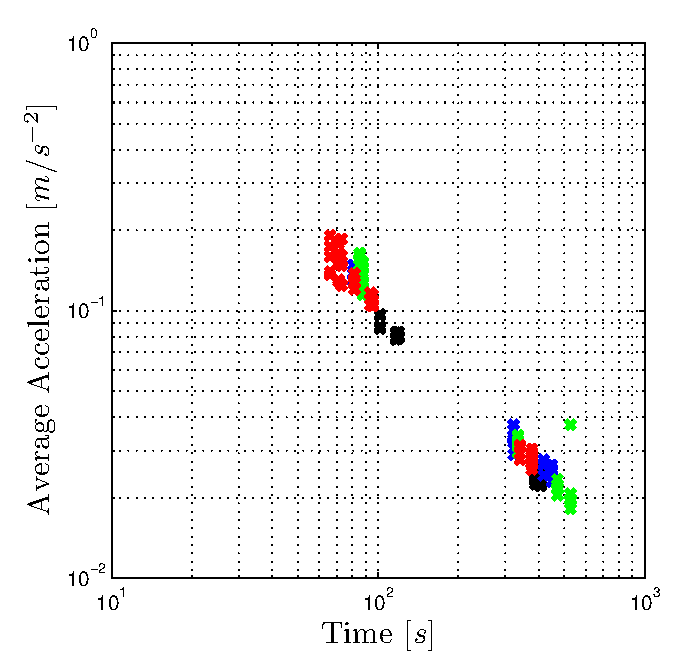
\includegraphics[width = \textwidth]{correlation/Control_Correlation_Time_Acc_Parametrization}
  \end{minipage}
  \hfill
  \begin{minipage}[t]{0.48\textwidth}
    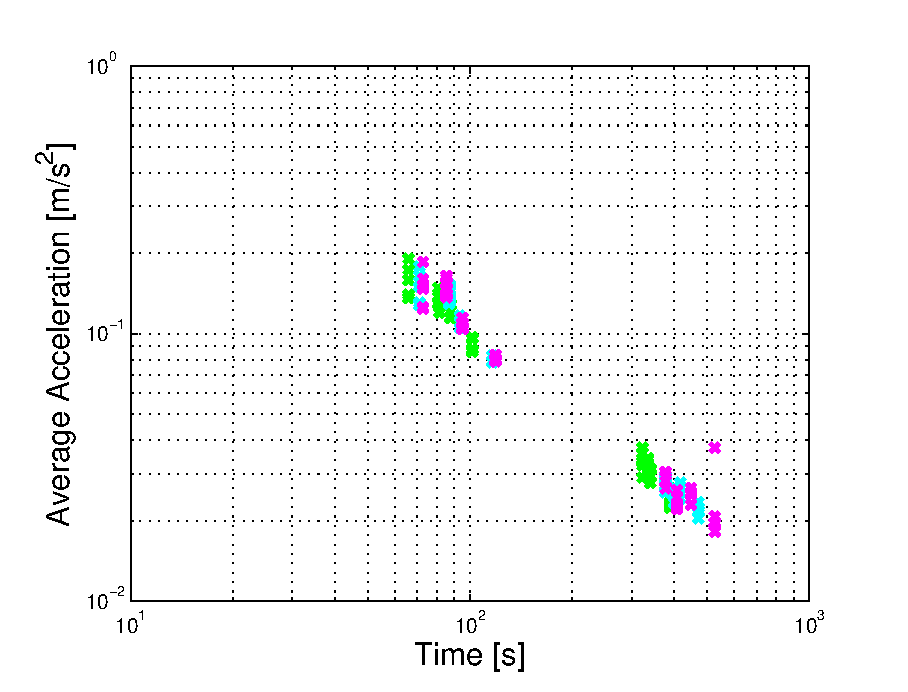
\includegraphics[width = \textwidth]{correlation/Control_Correlation_Time_Acc_SplineDegree}
  \end{minipage}
  \caption{Correlation between trajectory time length $T_p$ and average accelerations on trace. On the double logarithmic plot the correlation becomes clear. {\bf Left}: Different waypoint parametrizations uniform (black), chord length (blue), arc length (green) and centripetal (red). {\bf Right}: Different spline degrees cubic (green), quartic (cyan) and quintic (magenta).}
  \label{fig:correlation_time_acc}
\end{figure}

\begin{figure}[H]
  \begin{minipage}[t]{0.48\textwidth}
    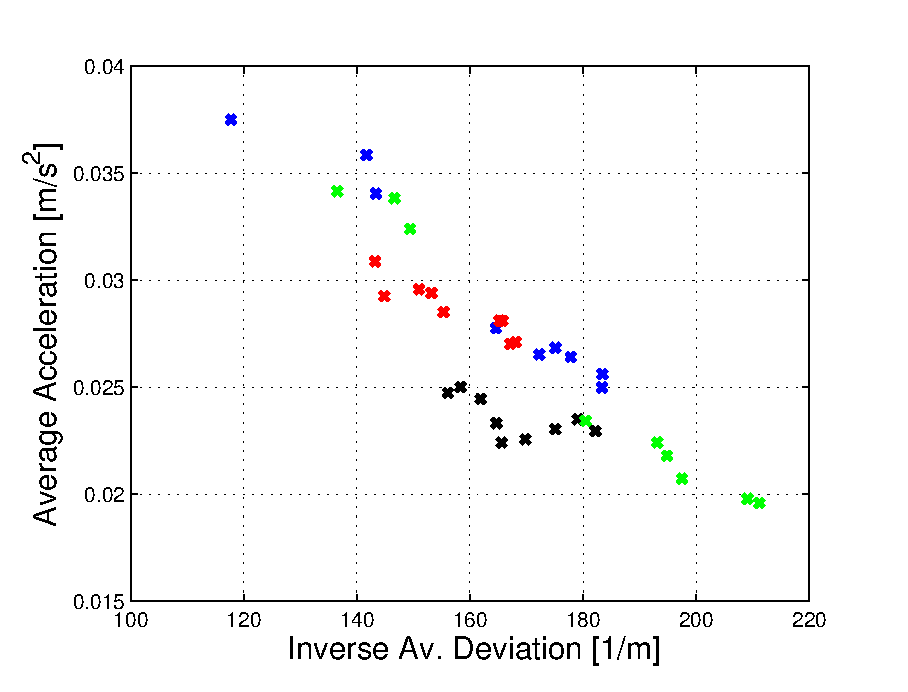
\includegraphics[width = \textwidth]{correlation/Control_Correlation_InvDev_Acc_Parametrization}
  \end{minipage}
  \hfill
  \begin{minipage}[t]{0.48\textwidth}
    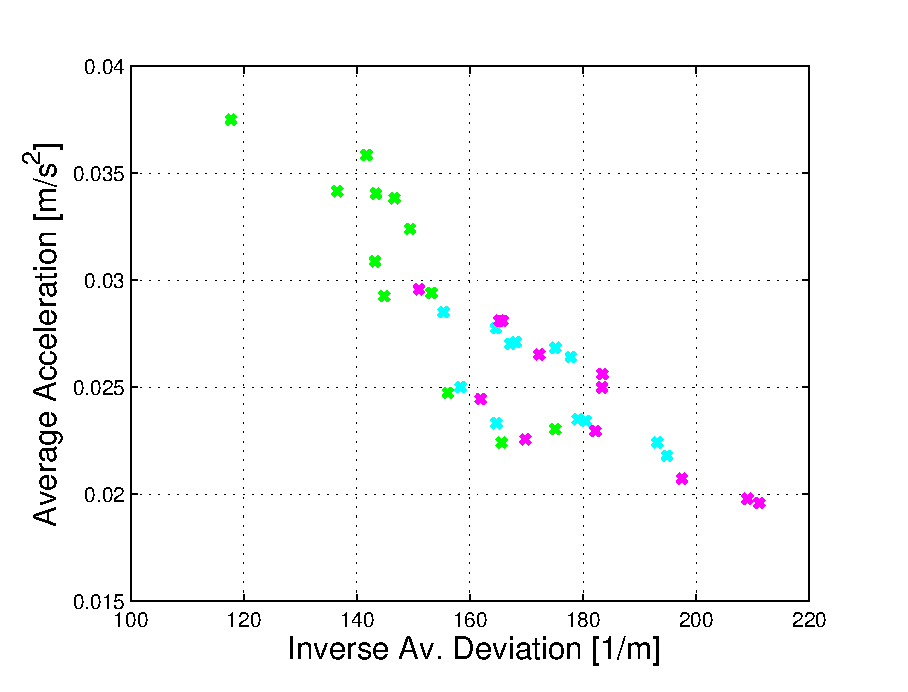
\includegraphics[width = \textwidth]{correlation/Control_Correlation_InvDev_Acc_SplineDegree}
  \end{minipage}
  \caption{Correlation between deviation between trajectory and trace. Data points from \textit{road} waypoints. {\bf Left}: Different waypoint parametrizations uniform (black), chord length (blue), arc length (green) and centripetal (red). {\bf Right}: Different spline degrees cubic (green), quartic (cyan) and quintic (magenta).}
  \label{fig:correlation_invdev_acc}
\end{figure}


\section{Discussion}
\label{sec:discussion}

\textit{The almost endless field of trajectories represents the individual needs for for trajectories within different situations. Before considering steering by waypoints, the criteria for a good fitting trajectory have to be elaborated. This can be very case-specific, as it depends not only on available system's actuation, but also on the way one sets the waypoints. The holonomic design of the system has to be considered as well as environmental obstacles at the scene. Suitable trajectory controllers will handle aaaaaaaaaaa\\ Therefore, geometrical design of the path has mainly to be considered. Dynamical aspect of the trajectory depends largely on the used controller..} HELLO?
